\section{Classical simulation}
\label{sec:classical}

In order to simulation a real chemical system, it is necessary to model the electrons of the molecules and their interactions.
This is usually achieved using quantum mechanical calculations, where the energy of the system is calculated by finding som approximate solution to the Schr\"{o}dinger equation.
However, quantum mechanical calculations are very computationally expensive, and are realistically limited to hundreds of atoms.
In order to simulate a soft matter system such as a lipid monolayer or polymer nanoparticles, it is necessary to simply the calculation being performed.
This leads to classical simulation, where mathematical functions are used to determined the potential energy of the system.
Classical simulations is used substantially in this work, in terms of both molecular dynamics simulations and energy minimisation methods (see Section \ref{sec:simulation}).
Therefore, it is necessary to introduce the underlying theory on which this method is defined.

\subsection{Potential models}
Potential modelling is a more computationally efficient method for the calcution of the potential energy of a chemical system.
A potential model consists of a series of mathematical functions that depend on the atomic positions, $\mathbf{r}$.
Each of the functions represents the potential energy of a different interaction for a given atom.
Broadly, these interactions can be split into bonded and non-bonded, such that the total energy may be described as follows,
%
\begin{equation}
  E_{\text{total}}(\mathbf{r}) = E_{\text{bonded}}(\mathbf{r}) + E_{\text{non-bonded}}(\mathbf{r})
\end{equation}
%
The total potential energy is then the sum of the potential energy for each of the individual atoms.

\subsubsection{Bonded terms}
The bonded terms are used to describe different aspects of chemical bonds.
These typically consist of bond stretchs, angle bends and dihedral torsions; within the OPLS2005 potential model \cite{Banks2005}, these interactions have the following mathematical form,
%
\begin{equation}
\begin{aligned}
  E_{\text{bonded}}(b, \theta, \phi) & = \sum_{\text{bonds}}K_b(b-b_0)^2 + \sum_{\text{angles}}K_{\theta}(\theta-\theta_0)^2 \\
  + \sum_{\text{dihedrals}} & \frac{1}{2}\big\{A_1[1 + \cos(\phi)] + A_2(1 - \cos(2\phi)] + A_3(1 + \cos(3\phi)]\big\},
\end{aligned}
\end{equation}
%
where, $K_b$ and $b_0$, $K_{\theta}$, $\theta_0$, and $A_1$, $A_2$, and $A_3$ are potential model dependent parameters for the bonds, angles, and dihedrals respectively, while $b$, $\theta$, and $\phi$ are the bond lengths, the size of the angles, and the size of the dihedrals that depend on the atom positions.
It can be seen that both the bond stretch and angle bend have harmonic functions, whereas the dihedral consists of a more complex multiple cosine function.
The values of the potential model dependent parameters are determined as outlined in Section \ref{sec:parameterisation}.

\subsubsection{Non-bonded terms}
The non-bonded terms are a series of functions that describe the potential energy of intermolecular interactions, such as eletrostatics and London dispersion forces.
The potential energy of the short-range interactions are usually modelled as a combination of the attractive London dispersion interaction and the repulsive exchange forces that arise from the Pauli exclusions principle \cite{Leach1996}.
These often forms such as shown below for the Lennard-Jones potential model \cite{LennardJones1924},
%
\begin{equation}
  E_{\text{non-boned}}(r) = E_{\text{repulsive}} + E_{\text{attractive}} = \frac{A}{r^{12}} - \frac{B}{r^6} = 4\varepsilon\Bigg[\bigg(\frac{\sigma}{r}\bigg)^{12} - \bigg(\frac{\sigma}{r}\bigg)^6\Bigg]
\end{equation}
%
where, $r$ is the distance between two particles, $A$ and $B$ are potential model dependent parameters, and $\sigma$ and $\epsilon$ are simple reformations of these parameters,
%
\begin{equation}
  A = 4\varepsilon\sigma^{12} \;\;\;\; B = 4\varepsilon\sigma^6.
\end{equation}
%
Fig.~\ref{fig:lj} shows each component of the Lennard-Jones potential model for atoms of argon, using parameters for $A$ and $B$ determined by Rahman \cite{Rahman1964}.
The Lennard-Jones is not the only potential model that may be used for the modelling of the short-range non-bonded interactions, others such as the Buckingham and Morse potentials exist \cite{Buckingham1938, Morse1929}.
However, the Lennard-Jones model has been used heavily in this work.
%
\begin{figure}
	\centering
	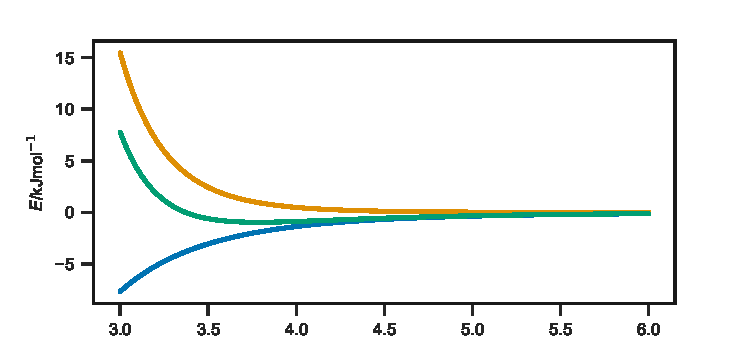
\includegraphics[width=0.85\textwidth]{theory/lj}
	\caption{The form of each component; attractive (blue), repulsive (orange), of the Lennard-Jones potential model (green) for argon, using parameters from Rahman \cite{Rahman1964}}
	\label{fig:lj}
\end{figure}
%

While the short-range interactions are accounted for by a function such as the Lennard-Jones potential model, the potential energy of the long-range electrostatic interactions are usually modelled, more consistently, using Coulomb's law for classical electrostatic interaction between point particles \cite{Coulomb1788, Coulomb1788a},
%
\begin{equation}
  E_{\text{Coulomb}}(r) = \frac{1}{4\pi\varepsilon_0}{\frac{q_iq_je^2}{r^2}},
\end{equation}
%
where, $r$ is the distance between the two particles, $\varepsilon_0$ is the dielectric permittivity of the vacuum, $e$ is the charge of the electron, and $q_i$ and $q_j$ are the electronic charges on each of the particles.





\subsection{Parameterisation}
\label{sec:parameterisation}
\subsection{Coarse-graining}
